\documentclass[aspectratio=169]{beamer}

\makeatletter
\def\input@path{{template/}}
\makeatother

\usetheme[dark]{uob}

\usepackage{booktabs}
\usepackage{array}

% Tighter list spacing
\setbeamertemplate{itemize items}[square]

% --- Image placeholder ------------------------------------------------------
%  A dashed, soft-gold framed box that stands in for artwork the author will
%  source separately. To drop in the real image later, replace the \imgph{..}
%  call with \includegraphics[width=\linewidth]{figures/your-image}.
%  Usage: \imgph[<width>]{<height>}{<caption>}  (width defaults to \linewidth)
\newcommand{\imgph}[3][\linewidth]{%
    \begin{tikzpicture}
        \node[draw=lightyellow, dashed, line width=0.8pt, rounded corners=3pt,
              fill=lightyellow!7, text=lightyellow, align=center,
              font=\scriptsize, inner sep=7pt, minimum height=#2,
              text width=\dimexpr#1-20pt\relax]
             {\textbf{[\,IMAGE\,]}\\[0.3em]\itshape #3};
    \end{tikzpicture}%
}

\title{Turning Churn Risk into Revenue}
\author{Daniel Adotey\\[0.5em]
\footnotesize A Proactive Retention Engine for Company A\\
\footnotesize GCI World 2026 (Matsuo--Iwasawa Lab, UTokyo) --- Final Assignment\\
\footnotesize Proof of Concept --- Data-Driven Business Proposal}
\date{\today}

% Clean PDF document properties. The \author macro carries subtitle lines for
% the custom title page, so set explicit, tidy metadata here to avoid leaking
% layout markup (\\[0.5em], etc.) into the PDF's Author field.
\hypersetup{
    pdftitle={Turning Churn Risk into Revenue},
    pdfauthor={Daniel Adotey},
    pdfsubject={GCI World 2026 (Matsuo-Iwasawa Lab, UTokyo) --- Final Assignment},
    pdfkeywords={customer churn, retention, telecom, machine learning, business proposal}
}

% --- Local title-page override: remove the UoB logo and soften ("blur") the
%     decorative line graphic on the right. Keeps the shared theme untouched. ---
\newlength{\tpmargin}\newlength{\tpheight}\newlength{\tpwidth}
% Draw a line as several stacked, low-opacity, round-capped strokes so it reads
% as a soft / blurred ray instead of a crisp 1pt line.
\newcommand{\blurray}[2]{%
    \draw[foregroundcolor, line cap=round, line width=26pt,  opacity=0.015] #1 -- #2;
    \draw[foregroundcolor, line cap=round, line width=19pt,  opacity=0.025] #1 -- #2;
    \draw[foregroundcolor, line cap=round, line width=13pt,  opacity=0.04 ] #1 -- #2;
    \draw[foregroundcolor, line cap=round, line width=8pt,   opacity=0.07 ] #1 -- #2;
    \draw[foregroundcolor, line cap=round, line width=4.5pt, opacity=0.12 ] #1 -- #2;
    \draw[foregroundcolor, line cap=round, line width=2pt,   opacity=0.20 ] #1 -- #2;
}
\setbeamertemplate{title page}{%
    \begin{tikzpicture}[remember picture, overlay]
        \fill[backgroundcolor] (current page.south west) rectangle (current page.north east);
        \setlength{\tpmargin}{0.5cm}
        \setlength{\tpheight}{\dimexpr\paperheight-2\tpmargin\relax}
        \setlength{\tpwidth}{\dimexpr\paperwidth-2\tpmargin\relax}
        \begin{scope}[shift={(current page.south west)}, xshift=\tpmargin, yshift=\tpmargin]
            \coordinate (center) at (\tpwidth, 0.33\tpheight);
            \node (author) at (0, 0.33\tpheight) [anchor=north west, color=foregroundcolor,
                font=\fontsize{12}{14}\selectfont, text width=0.67\tpwidth,
                inner xsep=0em, inner ysep=0.5em, align=left] {\insertauthor};
            \node (title) at (author.north west) [anchor=south west, color=foregroundcolor,
                font=\fontsize{24}{28}\selectfont, align=left, inner ysep=0.5em,
                inner xsep=0.5cm, xshift=-0.5cm] {%
                \begin{varwidth}{0.67\tpwidth}
                    \raggedright\hyphenpenalty=10000\exhyphenpenalty=10000
                    \titlefont \inserttitle
                \end{varwidth}};
            \coordinate (c1) at (0.88\tpwidth, \tpheight);
            \coordinate (c4) at (0.77\tpwidth, 0);
            \coordinate (cbl) at (0, 0);
            \blurray{(center)}{(c1)}
            \blurray{(center)}{(title)}
            \blurray{(center)}{(cbl)}
            \blurray{(center)}{(c4)}
        \end{scope}
    \end{tikzpicture}
}

\begin{document}

% ----------------------------------------------------------- 1. Title
\begin{frame}[plain]
    \titlepage
\end{frame}

% =========================================================== Market
\section{Market Context}

% ----------------------------------------------------------- 3. Market
\begin{frame}{In a mature market, growth comes from keeping customers}
    \begin{columns}[T]
    \begin{column}{0.56\textwidth}
        \begin{itemize}
            \item Mobile markets are \textbf{mature}: penetration exceeds 100\%
                  (multiple SIMs), so growth comes from \textbf{ARPU and retention},
                  not new subscribers.\hfill{\scriptsize[1]}
            \item Acquiring a subscriber costs roughly \textbf{5$\times$} more than
                  keeping one.\hfill{\scriptsize[2]}
            \item A \textbf{5\% lift in retention} can raise profit by
                  \textbf{25--95\%}.\hfill{\scriptsize[3]}
        \end{itemize}
        \begin{block}{The lever}
            Company A has 100{,}000 customers and an \$58.72 average monthly
            bill, but no in-house ML. Even a small drop in churn protects
            millions in recurring revenue.
        \end{block}
    \end{column}
    \begin{column}{0.44\textwidth}
        \begin{exampleblock}{Company A snapshot}
            \footnotesize
            \begin{tabular}{@{}lr@{}}
                Customers           & 100{,}000 \\
                Avg.\ monthly bill  & \$58.72 \\
                Avg.\ tenure        & 18.8 mo \\
                Avg.\ handset age   & 392 days \\
                Churn-risk signals  & $\approx$50\% \\
            \end{tabular}
        \end{exampleblock}
        {\scriptsize Our task: identify the business problem from the data and
        propose a solution the client can act on.}
        \vspace{0.3em}
        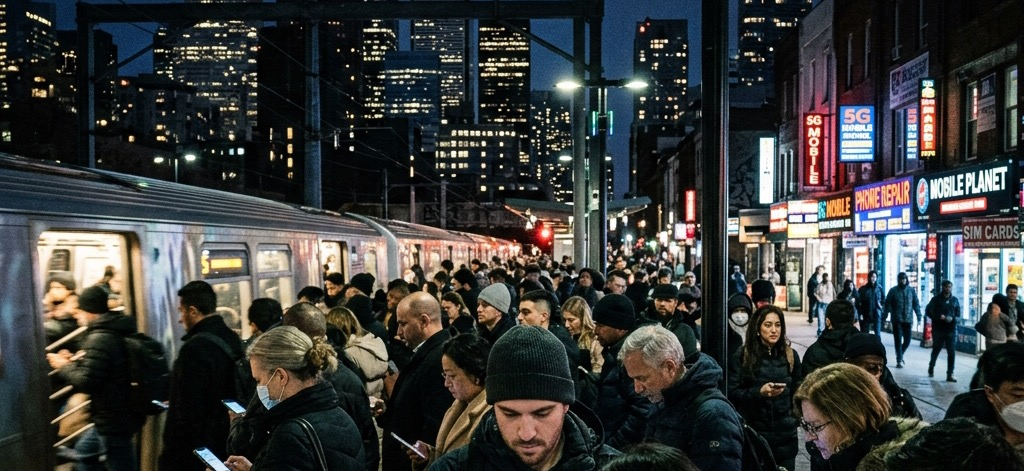
\includegraphics[width=\linewidth]{figures/slide3_market.png}
    \end{column}
    \end{columns}
\end{frame}

% =========================================================== Data
\section{Data \& Evidence}

% ----------------------------------------------------------- 5. Data + target
\begin{frame}{The data, and why churn is the right target}
    \begin{columns}[T]
    \begin{column}{0.52\textwidth}
        \begin{itemize}
            \item Two linked tables, joined 1:1 on \texttt{Customer\_ID}:
            \begin{itemize}\footnotesize
                \item \texttt{Client.csv} --- 100k $\times$ 50: tenure, plan,
                      handset, demographics
                \item \texttt{Record.csv} --- 100k $\times$ 51: monthly usage,
                      billing, call quality, \texttt{churn}
            \end{itemize}
            \item \textbf{Target = churn} (binary). It's the outcome the
                  business most wants to change, and the one tied to revenue.
            \item Classes are \textbf{near-balanced (49.6\% churn)} --- so both
                  \emph{accuracy} and \emph{AUC} are meaningful here.
        \end{itemize}
    \end{column}
    \begin{column}{0.48\textwidth}
        \centering
        
\includegraphics[width=\linewidth]{figures/churn_balance.png}
    \end{column}
    \end{columns}
\end{frame}

% ----------------------------------------------------------- 6. EDA drivers
\begin{frame}{What the data says drives churn}
    \begin{columns}[T]
    \begin{column}{0.6\textwidth}
        \centering
        
\includegraphics[width=\linewidth]{figures/churn_rate_by_feature.png}
    \end{column}
    \begin{column}{0.4\textwidth}
        Churn rate rises clearly with:
        \begin{itemize}
            \item \textbf{ageing handsets} (equipment age),
            \item \textbf{declining usage} (change in minutes),
        \end{itemize}
        and falls with engagement (customer-care contact, higher usage).
        \vspace{0.6em}
        \begin{block}{Why it matters}
            Each of these is something the business can \textbf{act on} ---
            unlike age or location.
        \end{block}
    \end{column}
    \end{columns}
\end{frame}

% ----------------------------------------------------------- 7. Diffuse signal
\begin{frame}{No single variable explains churn, so we need a model}
    \begin{columns}[T]
    \begin{column}{0.55\textwidth}
        \centering
        
\includegraphics[width=0.95\linewidth]{figures/correlation_heatmap.png}
    \end{column}
    \begin{column}{0.45\textwidth}
        \begin{itemize}
            \item Correlations with churn are \textbf{individually weak}
                  ($|r|<0.1$); revenue/usage columns are near-duplicates of
                  each other.
            \item Signal is \textbf{diffuse and non-linear}: simple rules
                  (like ``flag old phones'') only catch part of it.
        \end{itemize}
        \begin{exampleblock}{Implication}
            A multivariate model that combines weak signals will rank
            churn risk far better than any single threshold.
        \end{exampleblock}
    \end{column}
    \end{columns}
\end{frame}

% =========================================================== Modelling
\section{Modelling}

% ----------------------------------------------------------- 9. Approach
\begin{frame}{From business question to ML task}
    \begin{columns}[T]
    \begin{column}{0.5\textwidth}
        \textbf{Task.} Binary classification; output a per-customer
        \textbf{churn-probability score} the business can rank and target.
        \vspace{0.5em}

        \textbf{Feature engineering.}
        \begin{itemize}\footnotesize
            \item Dropped \texttt{Customer\_ID} (no predictive value).
            \item Encoded 21 categorical columns.
            \item Built \textbf{11 interpretable features} --- ratios, shares
                  and momentum: e.g.\ \texttt{usage\_momentum},
                  \texttt{rev\_per\_min}, \texttt{overage\_share},
                  \texttt{eqp\_per\_tenure}, \texttt{drops\_per\_call}.
        \end{itemize}
    \end{column}
    \begin{column}{0.5\textwidth}
        \textbf{Models compared.}
        \begin{itemize}\footnotesize
            \item \textbf{Logistic Regression} --- transparent linear baseline
                  (median-imputed, scaled).
            \item \textbf{XGBoost, CatBoost, HistGradientBoosting} ---
                  gradient-boosted trees; handle missing values and non-linear
                  interactions natively.
            \item \textbf{Rank-blend ensemble} of the three --- the final model.
        \end{itemize}
        \vspace{0.3em}
        \begin{block}{Metrics}
            \footnotesize \textbf{ROC-AUC} (ranking quality --- what targeting
            needs) plus \textbf{accuracy} (meaningful because classes are
            balanced), both via \textbf{5-fold stratified cross-validation}
            (honest out-of-fold predictions).
        \end{block}
    \end{column}
    \end{columns}
\end{frame}

% ----------------------------------------------------------- 10. Results (EXPLICIT)
\begin{frame}{Results: engineered features and the ensemble both lift AUC}
    \begin{columns}[T]
    \begin{column}{0.52\textwidth}
        \centering
        \footnotesize
        \begin{tabular}{@{}lccc@{}}
            \toprule
            \textbf{Model} & \textbf{Acc.} & \textbf{ROC-AUC} & \textbf{F1} \\
            \midrule
            Logistic Regression       & 0.596 & 0.633 & 0.587 \\
            XGBoost (no features)     & 0.641 & 0.697 & 0.642 \\
            XGBoost + features         & 0.648 & 0.706 & 0.645 \\
            CatBoost + features        & 0.648 & 0.704 & 0.646 \\
            \textbf{Ensemble (final)}  & \textbf{0.648} & \textbf{0.706} & \textbf{0.647} \\
            \bottomrule
        \end{tabular}
        \vspace{0.6em}
        \begin{block}{Chosen model}
            \footnotesize \textbf{Ensemble (CatBoost + XGBoost + HistGB) ---
            ROC-AUC 0.706, Accuracy 0.648}, by 5-fold cross-validation over all
            100{,}000 customers (vs.\ 0.50 for a random baseline). Feature
            engineering alone lifted AUC from 0.697 to 0.706.
        \end{block}
    \end{column}
    \begin{column}{0.46\textwidth}
        \centering
        
\includegraphics[width=0.96\linewidth]{figures/roc_comparison.png}
    \end{column}
    \end{columns}
\end{frame}

% ----------------------------------------------------------- 11. Levers
\begin{frame}{The model points to levers the business can pull}
    \begin{columns}[T]
    \begin{column}{0.55\textwidth}
        \centering
        
\includegraphics[width=\linewidth]{figures/feature_importance.png}
    \end{column}
    \begin{column}{0.45\textwidth}
        \footnotesize
        \begin{tabular}{@{}p{2.4cm}p{3.4cm}@{}}
            \toprule
            \textbf{Top driver} & \textbf{Business action} \\
            \midrule
            Equipment age, refurb, handset price & Proactive \textbf{handset upgrade} offers \\[0.3em]
            Usage \& revenue momentum & \textbf{Win-back} on usage decline \\[0.3em]
            Overage share, rev/min & \textbf{Right-plan} nudges \\
            \bottomrule
        \end{tabular}
        \vspace{0.5em}

        Gold bars are \textbf{engineered} features. Several reach the top
        tier (usage momentum is the \#4 driver), so the feature work paid
        off. {\scriptsize Tenure and account type rank high too, but as risk
        \emph{markers}, not levers.}
    \end{column}
    \end{columns}
\end{frame}

% =========================================================== Proposal
\section{Business Proposal}

% ----------------------------------------------------------- 13. Proposal + impact
\begin{frame}{Proposal: a Proactive Retention Engine}
    \begin{columns}[T]
    \begin{column}{0.5\textwidth}
        \textbf{How it works.} Score the base \textbf{monthly}; route the
        highest-risk customers to the matched offer (upgrade / win-back /
        re-plan).
        \vspace{0.4em}

        \textbf{Why targeting pays.} Most of the churn sits in a small slice:
        \begin{itemize}\footnotesize
            \item Top \textbf{20\%} by score $\Rightarrow$ \textbf{74\%} churn
                  density (\textbf{1.5$\times$} lift), capturing 30\% of all
                  churners.
            \item Retention spend stops subsidising the half who would stay
                  anyway.
        \end{itemize}
        \vspace{0.3em}
        
\includegraphics[width=\linewidth]{figures/slide13_retention.png}
    \end{column}
    \begin{column}{0.5\textwidth}
        \begin{exampleblock}{Year-1 impact (stated assumptions)}
            \footnotesize
            \begin{tabular}{@{}lr@{}}
                Target (top 20\%)        & 20{,}000 \\
                At-risk within target    & 14{,}880 \\
                Save rate (assumed 12\%) & 1{,}786 saved \\
                Revenue retained @\,\$705/yr & \textbf{\$1.26M} \\
                Program cost @\,\$40/offer   & \$0.80M \\
                \midrule
                \textbf{Net Year-1 benefit} & \textbf{$\approx$\$0.46M} \\
                \textbf{ROI}                & \textbf{$\approx$57\%} \\
            \end{tabular}
        \end{exampleblock}
        {\scriptsize Conservative: industry save rates run 10--20\%; benefit
        compounds in later years.}
    \end{column}
    \end{columns}
\end{frame}

% ----------------------------------------------------------- 14. Roadmap + risks
\begin{frame}{Roadmap and risks}
    \begin{columns}[T]
    \begin{column}{0.5\textwidth}
        \textbf{From PoC to production}
        \begin{enumerate}\footnotesize
            \item \textbf{Pilot} one region with an A/B holdout to measure true
                  uplift.
            \item \textbf{Integrate} monthly scoring into the CRM / offer engine.
            \item \textbf{Scale} nationally; refresh the model quarterly.
        \end{enumerate}
        \vspace{0.8em}
        \centering
        \begin{tikzpicture}[line cap=round, line join=round]
            % treasure-map style dashed trail, wandering left to right
            \draw[white, line width=3pt, dash pattern=on 4.5pt off 6pt]
                (0,-0.15)
                .. controls (0.90, 0.70) and (1.70, 0.65) .. (2.40,-0.10)
                .. controls (3.00,-0.70) and (3.90,-0.60) .. (4.50, 0.20)
                .. controls (5.05, 0.78) and (5.80, 0.50) .. (6.40, 0);
            % X marks the spot (solid)
            \draw[white, line width=3pt]
                (6.12,-0.28) -- (6.68,0.28)
                (6.12, 0.28) -- (6.68,-0.28);
        \end{tikzpicture}
    \end{column}
    \begin{column}{0.5\textwidth}
        \textbf{Risks \& mitigations}
        \begin{itemize}\footnotesize
            \item \textbf{Model drift} $\rightarrow$ scheduled retraining,
                  monitoring.
            \item \textbf{Wasted discounts} $\rightarrow$ move to
                  \textbf{uplift modelling} (target persuadables, not
                  sure-leavers).
            \item \textbf{Privacy} $\rightarrow$ consent-based use, no sensitive
                  attributes as levers.
        \end{itemize}
    \end{column}
    \end{columns}
    \vspace{0.4em}
    \begin{block}{Bottom line}
        On its own, the score changes nothing. The value is the \textbf{targeted
        retention program} it drives: 100k rows become a ranked action list
        with a defensible, positive ROI.
    \end{block}
\end{frame}

% ----------------------------------------------------------- 15. References
\begin{frame}{References}
    \footnotesize
    \begin{enumerate}
        \item GSMA. \textit{The Mobile Economy 2024}. GSMA Intelligence.
              (Market maturity \& ARPU-led growth.)
        \item Reichheld, F.\ F. \textit{The Loyalty Effect}. Harvard Business
              School Press, 2001. (Acquisition vs.\ retention cost.)
        \item Reichheld, F.\ F.\ \& Sasser, W.\ E. (1990). ``Zero Defections:
              Quality Comes to Services.'' \textit{Harvard Business Review}
              68(5), 105--111.
        \item Chen, T.\ \& Guestrin, C. (2016). ``XGBoost: A Scalable Tree
              Boosting System.'' \textit{Proc.\ KDD '16}, 785--794.
        \item Prokhorenkova, L.\ et al.\ (2018). ``CatBoost: unbiased boosting
              with categorical features.'' \textit{NeurIPS 31}.
        \item Pedregosa et al.\ (2011). ``Scikit-learn: Machine Learning in
              Python.'' \textit{JMLR} 12, 2825--2830.
        \item Company A telecom dataset, GCI World 2026 Final Assignment
              (Matsuo--Iwasawa Lab, UTokyo).
    \end{enumerate}
    \vfill
    {\fontsize{2}{3}\selectfont Portions of the code were developed with assistance from generative AI tools.}
\end{frame}

% =========================================================== Appendix
% Supplementary detail that did not fit the 15-slide deck. Body text is set
% at 5pt (< half the 11pt slide body font), per the supporting-notes brief.
% No \section here, to avoid the theme injecting an extra outline divider.

% ----------------------------------------------------------- A. Data & target
\begin{frame}{Appendix A: Data preparation, cleaning, and target choice}
    \begin{columns}[T]
    \begin{column}{0.5\textwidth}
        {\fontsize{5}{6}\selectfont
        \textbf{Source.} Two files joined 1:1 on \texttt{Customer\_ID} into a
        single 100{,}000\,$\times\sim$100 table. \textit{Client.csv} carries
        account-level fields (length-of-relationship \texttt{lor}, equipment age
        \texttt{eqpdays}, handset price \texttt{hnd\_price}, demographics, plan);
        \textit{Record.csv} carries mean monthly usage, billing and
        network-quality metrics plus the \texttt{churn} flag and \texttt{months}.

        \medskip
        \textbf{Why churn is the target.} The flag is unusually balanced
        ($\sim$50/50), which keeps accuracy interpretable, and it maps directly
        to the retention problem the business actually faces. Alternative targets
        (e.g.\ ARPU regression) were considered but answer a different question
        and would not produce a rankable at-risk list.

        \medskip
        \textbf{Identifier.} \texttt{Customer\_ID} is a unique key with no
        predictive content and is dropped before any modelling.
        \par}
    \end{column}
    \begin{column}{0.5\textwidth}
        {\fontsize{5}{6}\selectfont
        \textbf{Redundancy.} The $\sim$100 columns include several near-duplicate
        revenue and usage variants. Highly correlated columns were pruned to cut
        multicollinearity and noise without losing signal.

        \medskip
        \textbf{Missing values.} Columns that were heavily missing were dropped
        rather than imputed, since imputing a mostly-empty field invents data.
        The gradient-boosted trees handle remaining gaps natively; the logistic
        baseline alone used median imputation and standardisation.

        \medskip
        \textbf{Leakage guard.} Any field that could only be known \emph{after} a
        churn event was excluded. Tenure fields (\texttt{months}, \texttt{lor})
        are retained because they are known up front, but they are treated as
        risk \emph{markers}, not levers --- the business cannot act on them.

        \medskip
        \textbf{Key assumption.} The monthly means in \textit{Record.csv}
        represent a stable, comparable observation window across customers.
        \par}
    \end{column}
    \end{columns}
\end{frame}

% ----------------------------------------------------------- B. Features & model
\begin{frame}{Appendix B: Feature engineering and modelling detail}
    \begin{columns}[T]
    \begin{column}{0.5\textwidth}
        {\fontsize{5}{6}\selectfont
        \textbf{Engineered features (11).} Ratios, shares and momentum built to
        be interpretable to the business:
        \begin{itemize}
            \item \texttt{usage\_momentum} --- recent vs.\ baseline usage trend;
                  a sustained decline is an early churn signal.
            \item \texttt{rev\_per\_min} --- revenue per minute, a proxy for
                  plan fit.
            \item \texttt{overage\_share} --- overage charges as a share of the
                  bill; flags customers on the wrong plan.
            \item \texttt{eqp\_per\_tenure} --- equipment age relative to
                  tenure; isolates ageing-handset risk.
            \item \texttt{drops\_per\_call} --- dropped-call rate, a
                  network-quality proxy.
        \end{itemize}
        plus further ratio/share terms in the same family.

        \medskip
        \textbf{Categoricals.} 21 categorical columns encoded --- LabelEncoder as
        the baseline, with CatBoost additionally using native categorical
        handling.
        \par}
    \end{column}
    \begin{column}{0.5\textwidth}
        {\fontsize{5}{6}\selectfont
        \textbf{Models.} A transparent Logistic Regression baseline; XGBoost,
        CatBoost and HistGradientBoosting as non-linear learners; and a
        \textbf{rank-blend ensemble} of the three (averaging rank-normalised
        probabilities) as the final model, chosen for lower variance rather than
        a higher headline score.

        \medskip
        \textbf{Validation.} 5-fold stratified cross-validation over all 100{,}000
        rows; metrics are computed on honest out-of-fold predictions.
        \textbf{Fold-safety} is enforced: any group-aggregate or target-derived
        transform is fit on the fold-training slice only, then applied to the
        held-out fold and test --- so no validation information leaks into
        training.

        \medskip
        \textbf{Metric choice.} ROC-AUC is primary because targeting needs good
        \emph{ranking}, not a hard cut-off; accuracy and F1 are reported as
        secondary checks and are meaningful only because the classes are
        balanced.

        \medskip
        \textbf{Outcome.} Feature engineering lifted AUC from 0.697 to 0.706, and
        the ensemble matched the best single model (0.706) with more stable
        fold-to-fold behaviour.
        \par}
    \end{column}
    \end{columns}
\end{frame}

% ----------------------------------------------------------- C. Business case
\begin{frame}{Appendix C: Business-case assumptions and ROI derivation}
    \begin{columns}[T]
    \begin{column}{0.5\textwidth}
        {\fontsize{5}{6}\selectfont
        \textbf{Targeting logic.} The whole base is scored monthly; action is
        taken only on the \textbf{top 20\%} (20{,}000 of 100{,}000). That
        quintile carries a \textbf{74\% churn density} --- a 1.5$\times$ lift over
        the $\sim$50\% base rate --- and captures roughly 30\% of all churners.
        Concentrating spend here stops the program subsidising the half of
        customers who would stay anyway.

        \medskip
        \textbf{Year-1 arithmetic.}
        \begin{itemize}
            \item At-risk within target: $20{,}000 \times 74\% = 14{,}880$.
            \item Save rate \textbf{12\%} (assumed; industry runs 10--20\%)
                  $\Rightarrow 1{,}786$ customers saved.
            \item Revenue retained: $1{,}786 \times \$705/\text{yr}
                  \approx \$1.26\text{M}$.
            \item Program cost: $20{,}000 \times \$40/\text{offer}
                  = \$0.80\text{M}$.
            \item \textbf{Net Year-1} $\approx \$0.46$M; \textbf{ROI}
                  $\approx 57\%$.
        \end{itemize}
        \par}
    \end{column}
    \begin{column}{0.5\textwidth}
        {\fontsize{5}{6}\selectfont
        \textbf{Where the inputs come from.}
        \begin{itemize}
            \item \textbf{\$705/yr} is the annualised mean revenue per retained
                  customer, derived from the dataset's billing fields.
            \item \textbf{\$40/offer} is a blended cost across the three offer
                  types (handset upgrade / win-back / re-plan), charged against
                  the full targeted quintile, not just savers --- a deliberately
                  conservative treatment.
            \item The \textbf{12\%} save rate sits at the low end of the cited
                  industry range.
        \end{itemize}

        \medskip
        \textbf{Sensitivity.} At a 10\% save rate the program is near break-even;
        at 20\% the net benefit roughly doubles. The Year-1 figure also excludes
        downstream lifetime value --- saved customers persist into later years,
        so the steady-state return is higher.

        \medskip
        \textbf{Caveats.} This is a cross-sectional snapshot; it establishes
        \emph{correlation}, not proven causal uplift. The roadmap therefore
        starts with a regional pilot carrying an A/B holdout, which measures the
        true incremental save rate before any national scale-up.
        \par}
    \end{column}
    \end{columns}
\end{frame}

% ----------------------------------------------------------- D. EDA figures I
\begin{frame}{Appendix D: EDA, target balance and data quality}
    \begin{columns}[T]
    \begin{column}{0.5\textwidth}
        \centering
        
\includegraphics[width=0.95\linewidth]{figures/churn_balance.png}
        \par\vspace{0.4em}
        {\scriptsize Target is near-balanced (\textbf{49.6\% churned}) --- accuracy
        is interpretable and no resampling is needed, a key reason churn is a
        sound target.}
    \end{column}
    \begin{column}{0.5\textwidth}
        \centering
        
\includegraphics[width=0.95\linewidth]{figures/missingness.png}
        \par\vspace{0.4em}
        {\scriptsize A handful of columns are heavily empty; these are
        \textbf{dropped rather than imputed}, since imputing a mostly-empty field
        invents data.}
    \end{column}
    \end{columns}
\end{frame}

% ----------------------------------------------------------- E. EDA figures II
\begin{frame}{Appendix E: EDA, univariate churn signals}
    \begin{columns}[T]
    \begin{column}{0.5\textwidth}
        \centering
        
\includegraphics[width=0.95\linewidth]{figures/eqpdays_churn.png}
        \par\vspace{0.4em}
        {\scriptsize Churners carry \textbf{older handsets} --- equipment age is an
        \emph{actionable} retention lever (proactive upgrade offers), unlike
        tenure.}
    \end{column}
    \begin{column}{0.5\textwidth}
        \centering
        
\includegraphics[width=0.95\linewidth]{figures/churn_rate_by_feature.png}
        \par\vspace{0.4em}
        {\scriptsize Churn rate by octile of four key drivers: each moves
        monotonically, but \textbf{no single variable separates churn} ---
        motivating a multivariate model.}
    \end{column}
    \end{columns}
\end{frame}

% ----------------------------------------------------------- F. EDA + modelling
\begin{frame}{Appendix F: EDA correlations and the modelling AUC lift}
    \begin{columns}[T]
    \begin{column}{0.5\textwidth}
        \centering
        
\includegraphics[width=0.82\linewidth]{figures/correlation_heatmap.png}
        \par\vspace{0.4em}
        {\scriptsize Drivers correlate only \textbf{weakly with churn} and partly
        with each other --- supporting both the multivariate model and the
        pruning of near-duplicate columns.}
    \end{column}
    \begin{column}{0.5\textwidth}
        \centering
        
\includegraphics[width=0.95\linewidth]{figures/model_improvement.png}
        \par\vspace{0.4em}
        {\scriptsize 5-fold out-of-fold AUC: engineered features
        (\textbf{0.697$\rightarrow$0.706}) then the rank-blend ensemble each add
        lift.}
    \end{column}
    \end{columns}
\end{frame}

% ----------------------------------------------------------- G. Model diagnostics
\begin{frame}{Appendix G: Model diagnostics, ensemble confusion matrix}
    \centering
    
\includegraphics[height=0.66\textheight]{figures/confusion_matrix.png}
    \par\vspace{0.5em}
    {\scriptsize Final rank-blend ensemble at a 0.5 threshold (accuracy
    \textbf{0.648}). Errors are roughly balanced across stay / churn, consistent
    with the balanced target --- and for targeting we rank by score rather than
    apply this hard cut-off.}
\end{frame}

\end{document}
